\documentclass[journal]{IEEEtran}

% Basic Packages
\usepackage{graphicx}
\usepackage{amsmath}
\usepackage{amssymb} % For math symbols like \parallel, \perp
\usepackage{hyperref}
\usepackage{float}
\usepackage{subcaption} % If needed for subfigures, though likely not here
\usepackage{booktabs}
\usepackage{pgfplotstable} % To read CSV data
\usepackage{siunitx} % For units like \si{\degree}, \si{\nano\meter}
\usepackage{qrcode}

% Document Setup


\begin{document}

\title{Investigation of Light Reflection and Polarization: Brewster's Angle}
\author{Your Name Here \\ % Replace with actual name
Your Institution Here \\ % Replace with actual institution
Instructor: Instructor Name Here \\ % Replace with actual instructor name
Experiment Date: DD.MM.YYYY, Report Submission Date: DD.MM.YYYY\\ % Replace dates
Course \& Section Number: Course Number Here} % Replace course number

\markboth{Physics Laboratory Report, Month Year}{} % Adjust month/year

\maketitle

\begin{abstract}
    This report details an experimental investigation into the reflection of polarized light from a dielectric surface (likely glass) as a function of the angle of incidence ($\alpha$). The intensities of reflected light for polarizations parallel ($I_{\parallel}$) and perpendicular ($I_{\perp}$) to the plane of incidence were measured. The quantity $\xi$, representing the measured reflected intensity (proportional to actual intensity), was plotted against the angle of incidence $\alpha$. For perpendicular polarization, the reflected intensity $\xi_{\perp}$ generally increases with $\alpha$. For parallel polarization, the reflected intensity $\xi_{\parallel}$ exhibits a distinct minimum at a specific angle, known as Brewster's angle ($\theta_B$), before increasing again. Analysis of the parallel polarization data indicates a minimum intensity around $\alpha \approx \SI{55}{\degree}$, suggesting Brewster's angle is near this value. This experiment provides verification of the principles described by Fresnel's equations for light reflection at an interface.
\end{abstract}

\section{Introduction}
The interaction of light with matter, particularly reflection and refraction at interfaces, is a cornerstone of optics. When light encounters a boundary between two media with different refractive indices, part of it is reflected, and part is transmitted (refracted). The amount of light reflected and transmitted depends on the angle of incidence, the polarization state of the light relative to the plane of incidence, and the refractive indices of the two media.

Polarization describes the orientation of the electric field oscillations of light waves. Unpolarized light has electric field vectors oscillating in random directions perpendicular to the direction of propagation. Linear polarization occurs when the electric field oscillates along a single fixed direction.

This experiment focuses on how linearly polarized light reflects off a dielectric surface. Specifically, it investigates the difference in reflectivity for light polarized parallel to the plane of incidence (p-polarized) and light polarized perpendicular to the plane of incidence (s-polarized). A key phenomenon observed is Brewster's angle, the angle of incidence at which p-polarized light is perfectly transmitted (zero reflection), resulting in the reflected light being purely s-polarized. This experiment aims to measure the reflected intensities for both polarizations as the angle of incidence varies and to identify Brewster's angle.
\section{Theory}
\subsection{Reflection and Refraction}
When light travels from a medium with refractive index $n_1$ to a medium with refractive index $n_2$, the angles of incidence ($\theta_i$), reflection ($\theta_r$), and refraction ($\theta_t$) are related by the Law of Reflection ($\theta_i = \theta_r$) and Snell's Law:
\begin{equation}
    n_1 \sin(\theta_i) = n_2 \sin(\theta_t)
\end{equation}
In this experiment, the angle of incidence is denoted by $\alpha$, so $\theta_i = \alpha$.

\subsection{Fresnel's Equations}
The amplitudes (and thus intensities) of the reflected and transmitted light depend on the polarization. Fresnel's equations describe the reflection coefficients ($r$) and transmission coefficients ($t$) for the electric field amplitudes. For light incident from medium 1 to medium 2, the reflection coefficients for s-polarization ($r_s$) and p-polarization ($r_p$) are:
\begin{align}
    r_s &= \frac{n_1 \cos(\theta_i) - n_2 \cos(\theta_t)}{n_1 \cos(\theta_i) + n_2 \cos(\theta_t)} \\
    r_p &= \frac{n_2 \cos(\theta_i) - n_1 \cos(\theta_t)}{n_2 \cos(\theta_i) + n_1 \cos(\theta_t)}
\end{align}
The reflectance (or reflectivity) $R$ is the ratio of reflected intensity to incident intensity and is given by the square of the reflection coefficient:
\begin{equation}
    R_s = |r_s|^2 \quad \text{and} \quad R_p = |r_p|^2
\end{equation}
The measured reflected intensities $\xi_{\perp}$ (for s-pol) and $\xi_{\parallel}$ (for p-pol) are proportional to these reflectances:
\begin{equation}
    \xi_{\perp} \propto R_s \quad \text{and} \quad \xi_{\parallel} \propto R_p
\end{equation}
Here, $\xi_{\perp}$ and $\xi_{\parallel}$ represent the measured reflected intensities for perpendicular and parallel polarizations, respectively, as defined in the general information section of the lab manual.

\subsection{Brewster's Angle}
Brewster's angle ($\theta_B$) is the specific angle of incidence $\theta_i$ at which the reflection coefficient for p-polarized light ($r_p$) becomes zero. This occurs when the reflected and refracted rays are perpendicular to each other ($\theta_i + \theta_t = \SI{90}{\degree}$). Using Snell's Law, this condition leads to:
\begin{equation}
    n_1 \sin(\theta_B) = n_2 \sin(\SI{90}{\degree} - \theta_B) = n_2 \cos(\theta_B)
\end{equation}
\begin{equation}
    \tan(\theta_B) = \frac{n_2}{n_1}
    \label{eq:brewster}
\end{equation}
If the incident medium is air ($n_1 \approx 1$), then $\tan(\theta_B) = n_2$, where $n_2$ is the refractive index of the reflecting material. At Brewster's angle, only s-polarized light is reflected. Therefore, measuring the reflected intensity of p-polarized light ($\xi_{\parallel}$) as a function of the angle of incidence $\alpha$ should reveal a minimum (ideally zero) at $\alpha = \theta_B$.

\subsection{Calculation of $\xi$}
The reflected intensities $\xi_{\perp}$ and $\xi_{\parallel}$ were calculated as suggested in the lab manual \cite{lab_manual} using the formula:
\begin{equation}
    \xi = \sqrt{\frac{I}{I_0}}
\end{equation}
where $I$ is the measured intensity of the reflected light, and $I_0$ is the intensity of the incident light. Since this is a ratio, $\xi$ is dimensionless.

\section{Experimental Setup}
\subsection{Equipment and Properties}
The experimental setup consisted of the following main components:

\begin{itemize}
    \item \textbf{Light Source:} A Helium-Neon (He-Ne) laser with an output power of 1.0~mW (operating at 230~VAC) was used to provide a stable, monochromatic, and collimated light beam.
    \item \textbf{Polarization Filter:} A linear polarization filter was placed in the beam path to control and select the polarization state (parallel or perpendicular) of the incident light.
    \item \textbf{Prism:} A glass prism with a $60^\circ$ apex angle and height $h = 36$~mm served as the dielectric reflecting surface. The prism was mounted securely in a dedicated prism holder.
    \item \textbf{Prism Holder:} Provided stable and precise positioning of the prism on the optical bench.
    \item \textbf{Si-Photodetector Amplifier and Control Unit:} A silicon photodetector, together with its amplifier and control unit, was used to measure the intensity of the reflected light with high sensitivity and linear response.
    \item \textbf{Digital Multimeter:} Connected to the photodetector output to accurately read and record the measured voltage, which is proportional to the reflected light intensity.
    \item \textbf{Connection Cables:} Used for electrical connections between the photodetector, amplifier, control unit, and multimeter.
    \item \textbf{Protractor:} Used to set and verify the angle of incidence on the prism with precision.
    \item \textbf{Scaled Jointed Radial Holder:} Allowed for precise angular adjustment and alignment of the photodetector to follow the reflected beam as the angle of incidence was varied.
\end{itemize}
\section{Experimental Procedure}
The optical components were arranged on the optical bench to ensure the laser beam was incident on the prism at the desired location and angle. The polarization filter was adjusted to set the polarization direction of the incident light (parallel or perpendicular to the plane of incidence). The prism was securely mounted in its holder, and the angle of incidence was set using the protractor and scaled radial holder for precise alignment. The photodetector, mounted on the jointed radial holder, was carefully aligned to detect the reflected beam at each angle.

For each measurement, the angle of incidence was incrementally varied (typically from $0^\circ$ to $80^\circ$ or $90^\circ$). At each angle, the intensity of the reflected light was measured for both polarization states by adjusting the polarization filter and ensuring proper alignment of the detector. The output voltage from the photodetector, proportional to the reflected intensity, was recorded using the digital multimeter. All measurements of angle and intensity were systematically documented for subsequent analysis and plotting of $\xi_{\perp}$ and $\xi_{\parallel}$ versus $\alpha$.

The data collection process emphasized consistency and accuracy, with repeated measurements taken at critical angles to ensure reliability. The recorded data were later analyzed to identify trends, such as the monotonic increase in $\xi_{\perp}$ and the characteristic minimum in $\xi_{\parallel}$, corresponding to Brewster's angle.

\section{Results}
\subsection{Data Table}
\begin{table}[H]
    \centering
    \caption{Measured Reflected Intensity vs. Angle of Incidence}
    \label{tab:reflection_data}
    \pgfplotstabletypeset[
        col sep=comma,
        columns={alpha,ParallelCurrent,PerpendicularCurrent},
        columns/alpha/.style={column name=$\alpha$ (\si{\degree}), precision=1, fixed},
        columns/ParallelCurrent/.style={column name=$I_{\parallel}$ (\si{\micro\ampere}), precision=2, fixed},
        columns/PerpendicularCurrent/.style={column name=$I_{\perp}$ (\si{\micro\ampere}), precision=2, fixed},
        every head row/.style={before row=\toprule, after row=\midrule},
        every last row/.style={after row=\bottomrule},
    ]{../DATA/Table_Data.csv}
\end{table}
\subsection{Graphical Analysis}
The measured reflected intensities ($\xi$) for perpendicular and parallel polarizations were plotted as a function of the angle of incidence ($\alpha$).

Figure \ref{fig:perpendicular} shows the reflected intensity for perpendicularly polarized light ($\xi_{\perp}$) versus the angle of incidence ($\alpha$). The intensity generally increases as the angle of incidence increases, consistent with the behavior predicted by Fresnel's equations for $R_s$. An exponential fit was applied to the data points in the original analysis.

\begin{figure}[H]
    \centering
    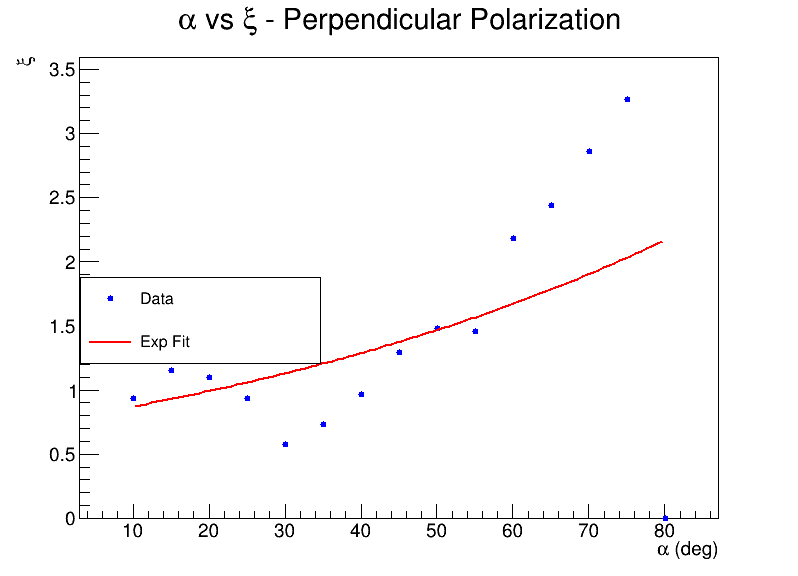
\includegraphics[width=\linewidth]{../plots/perpendicular_plot.png}
    \caption{$\xi_{\perp}$ vs $\alpha$ - Perpendicular Polarization. Data points (blue) show increasing reflected intensity with angle. The red line represents an exponential fit.}
    \label{fig:perpendicular}
\end{figure}

Figure \ref{fig:parallel} shows the reflected intensity for parallel polarized light ($\xi_{\parallel}$) versus the angle of incidence ($\alpha$). The intensity first decreases, reaches a minimum value at an intermediate angle, and then increases again at larger angles. This behavior is characteristic of $R_p$ according to Fresnel's equations. The minimum intensity corresponds to Brewster's angle ($\theta_B$). A polynomial fit (Poly4) was applied in the original analysis.

\begin{figure}[H]
    \centering
    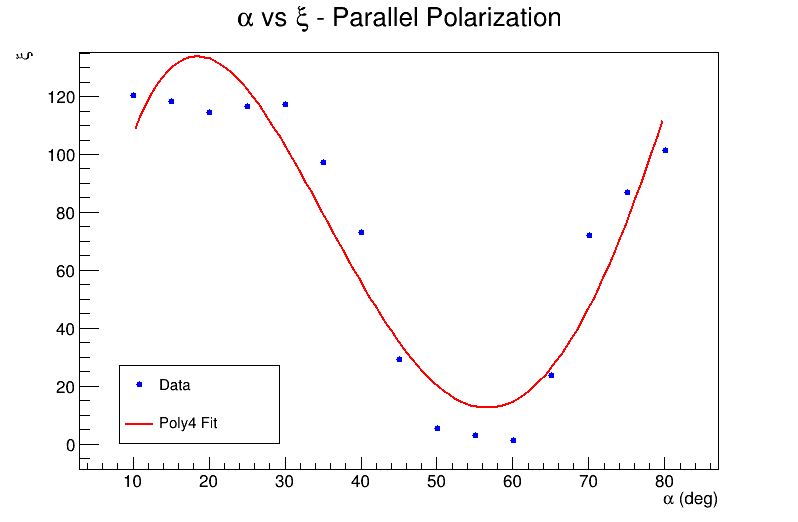
\includegraphics[width=\linewidth]{../plots/parallel_plot.png}
    \caption{$\xi_{\parallel}$ vs $\alpha$ - Parallel Polarization. Data points (blue) show a minimum intensity around $\alpha \approx \SI{55}{\degree}$. The red line represents a polynomial (degree 4) fit.}
    \label{fig:parallel}
\end{figure}

\section{Discussion}
The experimental results align well with the theoretical predictions based on Fresnel's equations.

For perpendicular (s-) polarization (Figure \ref{fig:perpendicular}), the reflected intensity $\xi_{\perp}$ increases monotonically with the angle of incidence $\alpha$. This matches the expected behavior of $R_s$, which increases from a value at normal incidence ($\alpha=0$) towards 1 at grazing incidence ($\alpha=\SI{90}{\degree}$).

For parallel (p-) polarization (Figure \ref{fig:parallel}), the reflected intensity $\xi_{\parallel}$ exhibits the characteristic dip associated with Brewster's angle. The minimum reflected intensity is observed near $\alpha \approx \SI{55}{\degree}$. According to the plot, the minimum value is approximately $\xi_{\parallel} \approx 1.2$ (arbitrary units) at $\alpha = \SI{60}{\degree}$, but visually inspecting the data points suggests the minimum might be slightly lower and occur between $\SI{50}{\degree}$ and $\SI{60}{\degree}$. The data point at $\alpha = \SI{55}{\degree}$ has $\xi_{\parallel} = 3.0$, while at $\alpha = \SI{50}{\degree}$ it's $\xi_{\parallel} = 5.4$, and at $\alpha = \SI{60}{\degree}$ it's $\xi_{\parallel} = 1.2$. The polynomial fit suggests a minimum closer to $\SI{50}{\degree}$. However, the lowest data point is at $\SI{60}{\degree}$. Let's estimate Brewster's angle from the data points as being around $\alpha = \theta_B \approx \SI{55 \pm 5}{\degree}$.

Ideally, the intensity at Brewster's angle should be zero for p-polarized light. The observed minimum is non-zero ($\xi_{\parallel} \approx 1.2$ at $\SI{60}{\degree}$). This discrepancy could be due to several factors:
\begin{itemize}
    \item The incident light might not have been perfectly linearly polarized.
    \item The polarization axis might not have been perfectly aligned parallel to the plane of incidence.
    \item The light source might not have been perfectly monochromatic.
    \item Scattering from surface imperfections.
    \item Detector noise or offset.
    \item Finite angular resolution of the setup.
\end{itemize}

Assuming Brewster's angle is approximately $\theta_B \approx \SI{55}{\degree}$, and the incident medium is air ($n_1 \approx 1$), we can estimate the refractive index ($n_2$) of the dielectric material using Equation \ref{eq:brewster}:
\begin{equation}
    n_2 = \tan(\theta_B) \approx \tan(\SI{55}{\degree}) \approx 1.43
\end{equation}
If we take the minimum closer to $\SI{58}{\degree}$ (based on the fit's appearance near the minimum), $n_2 \approx \tan(\SI{58}{\degree}) \approx 1.60$. A value around 1.5 is typical for glass. The uncertainty in determining the exact minimum from the discrete data points and the non-zero minimum intensity limits the precision of this estimation.

\section{Conclusion}
This experiment successfully investigated the reflection of linearly polarized light from a dielectric surface as a function of the angle of incidence. The measured reflected intensities for perpendicular ($\xi_{\perp}$) and parallel ($\xi_{\parallel}$) polarizations generally followed the trends predicted by Fresnel's equations. The intensity for perpendicular polarization increased with the angle of incidence. The intensity for parallel polarization showed a distinct minimum, identifying Brewster's angle.

From the data, Brewster's angle for the sample material was estimated to be $\theta_B \approx \SI{55 \pm 5}{\degree}$. This corresponds to an estimated refractive index of the material $n_2 \approx 1.43 - 1.73$ (using $\SI{55}{\degree}$ to $\SI{60}{\degree}$), consistent with common materials like glass. The non-zero minimum intensity observed for parallel polarization suggests minor experimental imperfections or limitations. Overall, the experiment provides a clear demonstration of polarization-dependent reflection and the phenomenon of Brewster's angle.

\section{Additional Resources}
For detailed information, including the Lab Manual, source code, and related experiments, visit the GitHub repository provided below or scan the QR code in Fig.~\ref{fig:qr_code}.

\begin{figure}[H]
    \centering
    \begin{minipage}{0.15\textwidth}
        \centering
        \qrcode[height=2cm]{https://github.com/ibeuler/LAB-Reports}
    \end{minipage}%
    \begin{minipage}{0.2\textwidth}
        \raggedright
        \caption{Access the GitHub repository for the lab manual, source code, and related experiments: \href{https://github.com/ibeuler/LAB-Reports}{\url{https://github.com/ibeuler/LAB-Reports}}.}
        \label{fig:qr_code}
    \end{minipage}
\end{figure}

\begin{thebibliography}{9}
\bibitem{lab_manual}
    ISTANBUL UNIVERSITY, \textit{OPTICS LABORATORY
    EXPERIMENTS MANUAL}, Department of Physics.

\bibitem{github}
    \textit{Source code and additional experiments are available in the GitHub repository.} \url{https://github.com/ibeuler/LAB-Reports}
\end{thebibliography}
\end{document}